\documentclass[pdflatex,compress,mathserif]{beamer}

%\usetheme[dark,framenumber,totalframenumber]{ElektroITK}
\usetheme[darktitle,framenumber,totalframenumber]{ElektroITK}

\usepackage[utf8]{inputenc}
\usepackage[T1]{fontenc}
\usepackage{lmodern}
\usepackage[bahasai]{babel}
\usepackage{amsmath}
\usepackage{amsfonts}
\usepackage{amssymb}
\usepackage{graphicx}
\usepackage{multicol}
\usepackage{lipsum}
\usefonttheme[onlymath]{serif}

\newcommand*{\Scale}[2][4]{\scalebox{#1}{$#2$}}%

\setbeamertemplate{caption}[numbered]

\title{METODE NUMERIK}
\subtitle{Pengantar Metode Numerik}

\author{Mifta Nur Farid}

\begin{document}

\maketitle

\section{Pengantar Metode Numerik}

\begin{frame}
	\frametitle{Apa itu Metode Numerik?}
	\begin{itemize}
		\item \textbf{Numerik:} berhubungan dengan angka.
		\item \textbf{Metode:} cara yang sistematis untuk menyelesaikan persoalan guna mencapai tujuan yang ditentukan.
		\item \textbf{Metode Numerik:} cara sistematis untuk menyelesaikan persoalan matematika dengan operasi angka (+, -, *, /).
	\end{itemize}
\end{frame}

\begin{frame}
	\frametitle{Contoh persoalan matematika}
	\begin{enumerate}
		\item Tentukan akar-akar persamaan polinom:
		\[ 23.4x^7 - 1.25x^6 + 120x^4 + 15x^3 - 120x^2- x + 100 = 0 \]
		\item Tentukan nilai $ x $ yang memenuhi persamaan:
		\[ \sqrt{27.8e^{5x} - \frac{1}{x}} = \cos^{-1}\frac{(120x^2 + \sqrt{2x})}{17x-65}\]
		\item Hitung nilai integral-tentu berikut:
		\[ \int_{1.2}^{2.5} \left( \sqrt{\left(45.3e^{7x}+\frac{100}{x}\right)^4} + \frac{4}{(x^2 + 1)} \right) dx \]
	\end{enumerate}
\end{frame}

\begin{frame}
	\begin{enumerate}
		\setcounter{enumi}{3}
		\item Diberikan persamaan differensial biasa (PDB) dengan sebuah nilai awal:
		\[ 150y'' + 2y't = \frac{\sqrt{\ln(21t+40)y}}{t^2} + 120;~y(0)=1 \]
		Hitung nilai $ y $ pada saat $ t = 1.8 $
	\end{enumerate}
\end{frame}

\begin{frame}
	\begin{enumerate}
		\setcounter{enumi}{4}
		\item Selesaikan sistem persamaaan linear:
		\begin{align*}
			1.2a - 3b -  12c + 12d + 4.8e - 5.5f	+ 100g  &= 18 \\
			0.9a + 3b -    c + 16d +   8e -   5f	-  10g  &= 17 \\
			4.6a + 3b -   6c -  2d +   4e + 6.5f	-  13g  &= 19 \\
			3.7a - 3b +   8c -  7d +  14e + 8.4f	+  16g  &=  6 \\
			2.2a + 3b +  17c +  6d +  12e - 7.5f	+  18g  &=  9 \\
			5.9a + 3b +  11c +  9d -   5e -  25f	-  10g  &=  0 \\
			1.6a + 3b + 1.8c + 12d -   7e + 2.5f	+    g  &= -5
		\end{align*}
	\end{enumerate}
\end{frame}

\begin{frame}
	\frametitle{Cara penyelesaian \\
		persoalan matematika}
	\begin{itemize}
		\item Cara penyelesaian persoalan matematika ada 2:
		\begin{enumerate}
			\item \textbf{Secara analitik:} menggunakan rumus dan teoremayang sudah baku di dalam matematika $\rightarrow$ metode analitik.
			\item \textbf{Secara numerik:} menggunakan pendekatan aproksimasi untuk mencari solusi hanya dengan operasi aritmatika biasa $\rightarrow$ metode numerik.
		\end{enumerate}
	\end{itemize}
\end{frame}

\begin{frame}
	\frametitle{Contoh 1}
	$ x^2 - 6x + 8 = 0 \rightarrow $ Carilah akar-akarnya! \\
	\begin{enumerate}
		\item Metode analitik: faktorkan menjadi $$ (x-4)(x-2) = 0 $$
		\begin{align*}
			x - 4 = 0 &\rightarrow x_1 = 4 \\
			x - 2 = 0 &\rightarrow x_2 = 2
		\end{align*}
	\end{enumerate}
\end{frame}

\begin{frame}
	\begin{enumerate}
		\setcounter{enumi}{1}
		\item Metode Numerik: Diketahui sebuah akar terletak di dalam selang [3, 6] $\rightarrow$ mengapa?
		
		\begin{figure}
			\centering
			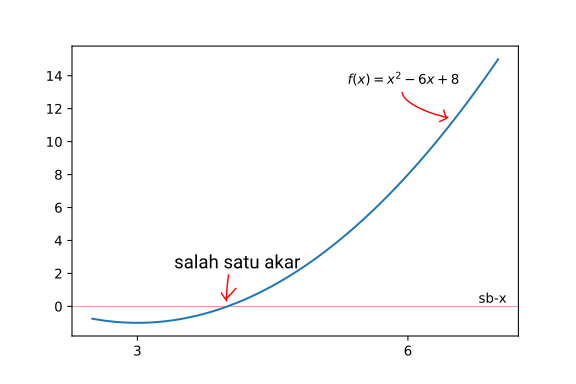
\includegraphics[width=0.8\linewidth]{img/img001}
		\end{figure}
		
	\end{enumerate}
\end{frame}

\begin{frame}
	Pendekatan sederhana mencari akar adalah secara iteratif dengan \textbf{metode titik tengah} (\textit{bisection method})
	
	\begin{enumerate}
		\item bagi selang $ [a,b] $ menjadi dua dengan titik tengah, $ c = (a + b) / 2 $
		\item ada dua sub-selang: $ [a, c] $ dan $ [c, b] $. Pilih selang iterasi yang baru dengan syarat nilai fungsi di ujung selang berbeda tanda.
		\item ulangi langkah 1 dan 2 sampai ukuran selang $ < \varepsilon$ (epsilon adalah nilai yang sangat kecil yang menyatakan toleransi kesalahan akar yang diinginkan, misalnya $\varepsilon$ = 0.001, 000001, dsb
	\end{enumerate}
\end{frame}

\begin{frame}
	\begin{center}
		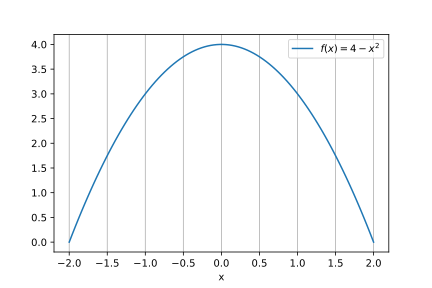
\includegraphics[width=\linewidth]{img/img002}
	\end{center}
\end{frame}

\begin{frame}
	\begin{itemize}
		\item Mencari akar $ f(x) = x^2 - 6x + 8 = 0 $ di dalam selang $ [3, 6] $ dengan $ \varepsilon = 0.0005 $
		
		\begin{center}
			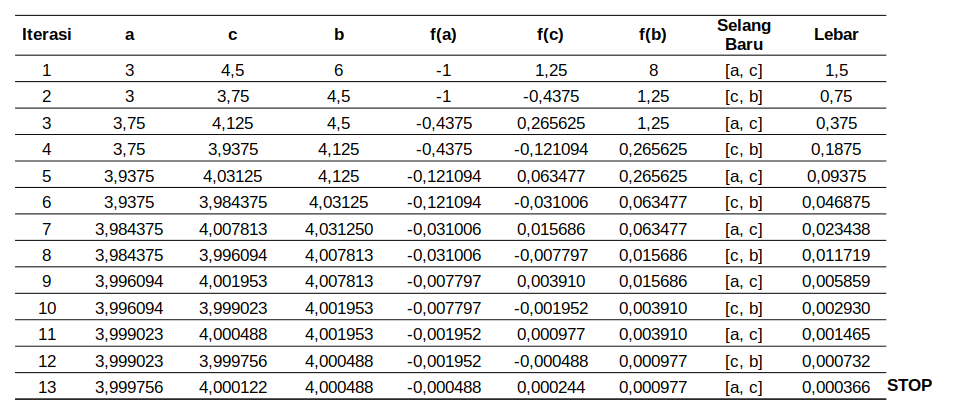
\includegraphics[width=\linewidth]{img/tab001}
		\end{center}
		
		\item Aproksimasi akar $\approx$ 4.000122
	\end{itemize}
\end{frame}

\begin{frame}
	\frametitle{Contoh 2}
	
	Hitung integral $ \int_{-1}^{1} (4 - x^2) dx $
	
	\begin{enumerate}
		\item Metode analitik.
		
		Persamaan: 
		\begin{equation*}
			\int ax^n dx = \frac{1}{n+1}ax^{n+1} + C
		\end{equation*}
		
		\begin{align*}
			\int_{-1}^{1} (4 - x^2) dx &= \left[4x - \frac{1}{3}x^3\right]^{x=1}_{x=-1} \\
			&=\left[ 4(1) - \frac{1}{3}(1) \right] - \left[ 4(-1) - \frac{1}{3}(-1) \right] \\
			&= \frac{22}{3} = 7.33
		\end{align*}
	\end{enumerate}
	
\end{frame}

\begin{frame}
	\begin{enumerate}
		\setcounter{enumi}{1}
		\item Metode numerik. \\
		
		Nilai integral = luas daerah di bawah kurva
		
		\begin{center}
			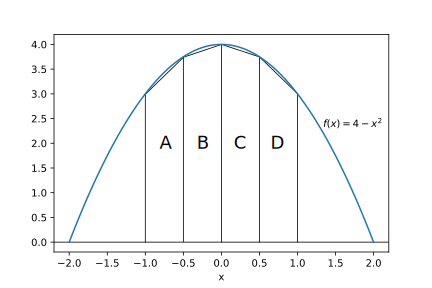
\includegraphics[width=0.6\linewidth]{img/img003}
		\end{center}
		
		Luas trapesium = (jumlah sisi sejajar $\times$ tinggi) / 2
	\end{enumerate}
\end{frame}

\begin{frame}
	\begin{align*}
		\text{Nilai integral} \approx&~ \text{Total luas trapesium} \\
		\int_{-1}^{1} (4-x^2) dx  \approx&~  A + B + C + D \\
		\approx&~ \{([ f(-1) + f(-0.5) ] \times 0.5) / 2 \} \\
		&+ \{([ f(-0.5) + f(0) ] \times 0.5) / 2 \} \\
		&+ \{([ f(0) + f(0.5) ] \times 0.5) / 2 \} \\
		&+ \{([ f(0.5) + f(1) ] \times 0.5) / 2 \} \\
		\approx&~ 0.5/2 \{ f(-1) + 2f(-0.5) + 2f(0) + 2f(0.5) + f(1) \} \\
		\approx&~ 0.5/2 \{ 3 + 7.5 + 8 + 7.5 + 3 \} \\
		\approx&~ 7.25
	\end{align*}
\end{frame}

\begin{frame}
	\frametitle{Perbedaan analitik dan numerik}
	\begin{itemize}
		\item Perbedaan solusi antara metode analitik dengan metode numerik:
		\begin{itemize}
			\item Solusi dengan metode analitik: eksak (tepat tanpa ada kesalahan)
			\item Solusi dengan metode numerik: hampiran atau aproksimasi (tidak tepat sama dengan solusi eksak, selalu ada kesalahan
		\end{itemize}
		\item Kesalahan dalam solusi numerik disebut galat (error)
		\item Galat dapat diperkecil dengan mengubah parameter di dalam metode numerik (misalnya $\varepsilon$, lebar trapesium, dsb)
	\end{itemize}
\end{frame}

\begin{frame}
	\frametitle{Kelebihan metode numerik}
	\begin{itemize}
		\item Metode numerik dapat menyelesaikan persoalan matematika yang tidak dapat diselesaikan dengan metode analitik.
		\item Apakah metode analitik mampu mencari akar persamaan di bawah ini?
		\[ \sqrt{27.8e^{5x} - \frac{1}{x}} = \cos^{-1}\frac{(120x^2 + \sqrt{2x})}{17x-65}\]
		\item Apakah metode analitik mampu mencari nilai integral berikut ini?
		\[ \int_{1.2}^{2.5} \left( \sqrt{\left(45.3e^{7x}+\frac{100}{x}\right)^4} + \frac{4}{(x^2 + 1)} \right) dx \]
		\item \textbf{Metode numerik mampu menyelesaikan persoalan di atas! }
	\end{itemize}
\end{frame}

\begin{frame}
	\begin{itemize}
		\item Metode numerik membutuhkan banyak operasi aritmetika yang berulang.
		\item Oleh karena itu, komputer berguna untuk membantu perhitungan. Komputer menjadi kebutuhan yang penting dalam metode numerik.
		\item Metode numerik pada dasarnya adalah suatu algoritma sehingga dapat diprogram.
		\item Bahasa pemrograman yang akan digunakan dalam perkuliahan ini adalah \textbf{Python} dengan IDE (\textit{integrated development environtments}) \textbf{Spyder} atau \textbf{Google Colab} (jika selalu memiliki akses internet)
		\begin{itemize}
			\item Spyder: \href{https://github.com/spyder-ide/spyder/releases/latest/download/Spyder_64bit_full.exe}{\beamergotobutton{Link}}
			\item Google colab: \href{https://colab.research.google.com/}{\beamergotobutton{Link}}
		\end{itemize}
	\end{itemize}
\end{frame}

\begin{frame}
	\begin{itemize}
		\item Tahapan penyelesaian persoalan secara numerik:
		\begin{enumerate}
			\item Pemodelan
			\item Penyederhanaan model
			\item Formulasi numerik: menentukan metode numerik yang dipakai dan membuat algoritma penyelesaian
			\item Pemrograman: coding
			\item Pengujian: tes dengan data uji
			\item Evaluasi: menganalisis hasil numerik
		\end{enumerate}
		\item Tahap 1 dan 2 adalah pekerjaan ahli yang sesuai dengan bidangnya.
		\item Tahap 3 dan 4 adalah tugas \textit{electrical engineering};
		\item Tahap 5 dan 6 melibatkan \textit{electrical engineering} dan ahli yang sesuai dengan bidangnya
		
	\end{itemize}
\end{frame}

% ----------------------------------------------------------------------------
\section{Kontrak Perkuliahan}

\begin{frame}
	\frametitle{Kontrak Perkuliahan}
	Rencana Pembelajaran Perkuliahan (RPS): \href{../../../silabus/TE201406_Metode_Numerik_RPS_2023.pdf}{\beamergotobutton{Link}}
\end{frame}


\end{document}
